\documentclass{beamer}
\usetheme{Madrid}
\usecolortheme{default}
\useoutertheme{split}
\setbeamertemplate{headline}{}
\useinnertheme{circles}
\usepackage{xcolor}
\usepackage{mathrsfs} 
\usepackage{bbm}
\usepackage{amsmath}
\usepackage{hyperref}
\usepackage{animate} 
\usepackage[ruled,vlined,noend]{algorithm2e} 
\usepackage{caption}
\usepackage{subcaption}
\usepackage{graphicx} 
\usepackage{comment}
\usepackage{booktabs}
\usepackage{array} 
\usepackage{appendixnumberbeamer}
\usepackage{tikz} 
\usetikzlibrary{arrows.meta,positioning,calc,decorations.pathreplacing} 
\captionsetup[figure]{font=tiny}

% --- Template Definitions ---
\DeclareMathOperator*{\argmax}{arg\,max}
\DeclareMathOperator*{\argmin}{arg\,min}

% Colors
\definecolor{CSred}{RGB}{160,32,60}
\definecolor{CSgrey}{RGB}{136,121,150}
\definecolor{UPSred}{RGB}{97,21,58}
\definecolor{FitBlue}{RGB}{35,104,166}
\definecolor{DesignOrange}{RGB}{213,94,0}

% Theme adjustments
\setbeamercolor{titlelike}{bg=CSred}
\setbeamerfont{title}{series=\bfseries}
\setbeamercolor{palette primary}{bg=CSred,fg=white}
\setbeamercolor{palette secondary}{bg=CSred,fg=white}
\setbeamercolor{palette tertiary}{bg=CSgrey,fg=white}
\setbeamercolor{palette quaternary}{bg=CSgrey,fg=white}
\setbeamercolor{structure}{fg=CSgrey}
\setbeamercolor{alerted text}{fg=CSred}
\setbeamertemplate{navigation symbols}{}

\usepackage[
backend=biber,
style=numeric,
sorting=none,
maxcitenames=1,
mincitenames=1
]{biblatex}
\addbibresource{bibliography.bib}
\renewcommand*{\bibfont}{\footnotesize}

% --- Presentation helpers ---
\newcommand{\CSonly}{\colorbox{CSred}{\textcolor{white}{\scriptsize\bfseries CS ONLY}}}
\newcommand{\takeaway}[1]{%
  \begin{beamercolorbox}[rounded=true,sep=0.7ex,wd=\linewidth]{palette primary}
    \centering\bfseries #1
  \end{beamercolorbox}}
\newcommand{\softbox}[2]{%
  \begin{beamercolorbox}[rounded=true,sep=0.8ex,wd=\linewidth]{#1}#2\end{beamercolorbox}}
\newcommand{\slidesource}[1]{%
  \par\vspace{0.2ex}{\raggedleft\scriptsize\color{gray}#1\par}}
\newcommand{\fitparam}[1]{\textcolor{FitBlue}{#1}}
\newcommand{\designparam}[1]{\textcolor{DesignOrange}{#1}}
\newcommand{\sectiondividercontent}[2]{%
  \centering
  \vfill
  {\color{CSgrey}\Large\bfseries Section #1}\par
  \vspace{0.8em}
  {\color{CSred}\Huge\bfseries #2}\par
  \vspace{0.8em}
  {\color{CSgrey}\rule{0.42\textwidth}{1.2pt}}\par
  \vfill
}
\newcommand{\validationdiagram}[1]{%
  \resizebox{\linewidth}{!}{%
  \begin{tikzpicture}[
      box/.style={rectangle,draw,rounded corners=4pt,minimum width=3.0cm,minimum height=1.05cm,align=center,font=\small},
      arr/.style={-{Stealth[length=6pt]},thick},
      darr/.style={{Stealth[length=5pt]}-{Stealth[length=5pt]},dashed,thick,color=gray!75}
    ]
    % A fixed bounding box keeps every block in exactly the same position
    % throughout the progressive explanation.
    \path[use as bounding box] (-1.65,-3.25) rectangle (9.65,2.25);
    \node[box,fill=blue!8] (ref) at (0,0) {Reference model\\population truth $\theta^*$};
    \ifnum#1>1
      \node[box,fill=orange!12] (sim) at (4,0) {Synthetic cohort $m$\\$y$, event time, indicator};
      \draw[arr] (ref)--(sim);
      \node[font=\scriptsize] at ($(ref.east)!0.5!(sim.west)+(0,0.75)$) {simulate};
    \fi
    \ifnum#1>2
      \node[box,fill=green!10] (fit) at (8,0) {Fresh fitted model\\$\hat\theta^{(m)}$};
      \draw[arr] (sim)--(fit);
      \node[font=\scriptsize] at ($(sim.east)!0.5!(fit.west)+(0,0.75)$) {fit};
      \draw[decorate,decoration={brace,amplitude=6pt,raise=15pt}]
        (sim.north west)--(fit.north east)
        node[midway,above=13pt,font=\footnotesize\itshape,fill=white,inner sep=1.5pt]{repeat $M$ times};
    \fi
    \ifnum#1>3
      \node[box,fill=blue!8] (true) at (4,-2.1) {True sampled effects\\$\tau_i,\xi_i,\ldots$};
      \node[box,fill=CSred!10] (perso) at (8,-2.1) {Personalised effects\\$\hat\tau_i,\hat\xi_i,\ldots$};
      \draw[arr] (sim)--node[left,font=\footnotesize]{retain truth}(true);
      \draw[arr] (fit)--node[right,font=\footnotesize]{personalise}(perso);
    \fi
    \ifnum#1>4
      \draw[darr] (ref.north) .. controls +(0,1.75) and +(0,1.75) ..
        node[pos=0.5,above,font=\footnotesize,color=black]{RB, RRMSE} (fit.north);
      \draw[darr] (true)--node[midway,below=17pt,font=\footnotesize,color=black]{ICC, Pearson's $r$}(perso);
    \fi
  \end{tikzpicture}}}
\setbeamercolor{softgrey}{bg=CSgrey!12,fg=black}
\setbeamercolor{softred}{bg=CSred!10,fg=black}
\setbeamercolor{softgreen}{bg=green!10,fg=black} 
\setbeamercolor{fitinput}{bg=FitBlue!16,fg=black}
\setbeamercolor{designinput}{bg=DesignOrange!16,fg=black}

% --- Metadata ---
\title[Paris Brain Institute (ICM) -- INRIA ARAMIS]{Developing simulation and statistical evaluation tools for a nonlinear mixed-effects model}  
\subtitle{Extending and validating the joint model in Leaspy}
\author[Jean-Vincent Martini]{Jean-Vincent Martini}
\institute[ICM -- INRIA ARAMIS]{Paris Brain Institute (ICM) -- INRIA ARAMIS\\[0.25em]
  End-of-studies internship, April--September 2026}
\date{September 2026}
\titlegraphic{
  
\includegraphics[height=1.5cm]{logos/logoICM.png}\hspace{1.1cm}
  
\includegraphics[height=1.5cm]{logos/logoCS.png}\hspace{1.1cm}
  
\includegraphics[height=1.5cm]{logos/logoMVA.jpg}
}

\begin{document} 

\frame{\titlepage}

% ============================================================================
\section{Motivation and context}

\begin{frame}[plain,noframenumbering]
  \sectiondividercontent{1}{Motivation and context}
\end{frame}

\begin{frame}{Longitudinal data: repeated observations over time}
  \begin{columns}[T,onlytextwidth]
    \begin{column}{0.40\textwidth}
      \begin{itemize}
        \item The \alert{same patient $i$} is observed at several chronological ages $t$.
        \item Visits can be sparse, irregular, unbalanced, and partially missing.
        \item Repeated measurements from one patient are correlated.
      \end{itemize}

      \vspace{0.7em}
      
    \end{column}
    \begin{column}{0.57\textwidth}
      \centering
      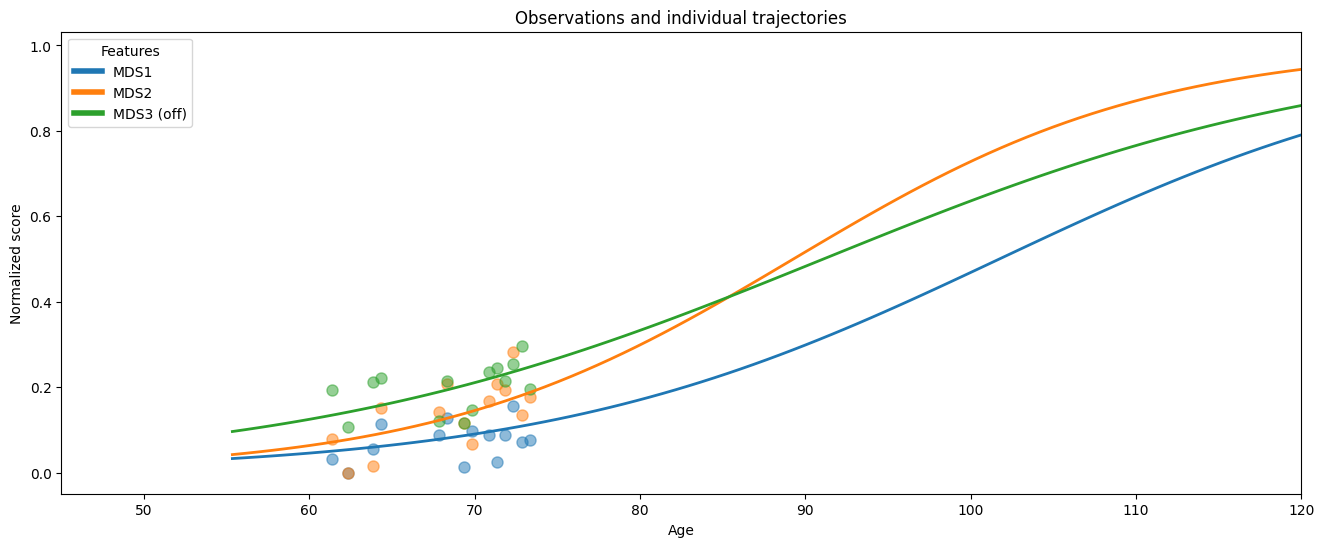
\includegraphics[width=\linewidth]{figures/obs_example.png}

      \scriptsize Dots: observations at successive visits.\quad
      Curves: personalised trajectories.
    \end{column}
  \end{columns}

  \vfill
  \softbox{softgrey}{
        We write $y_i(t)$ for the clinical scores observed for patient $i$ at age $t$.\\
        \textbf{Nonlinear mixed-effects models} combine a population trajectory
        with patient-specific deviations.
      }
  \takeaway{Reconstruct disease dynamics from short, heterogeneous follow-ups.}
\end{frame}

\begin{frame}{Why simulation is indispensable here}
  \begin{columns}[T,onlytextwidth]
    \begin{column}{0.31\textwidth}
      \softbox{softgrey}{
        \centering\textbf{Known truth}\\[0.4em]
        \small Real cohorts never reveal a patient's exact progression stage or patient-specific parameters.
      }
    \end{column}
    \begin{column}{0.31\textwidth}
      \softbox{softred}{
        \centering\textbf{Controlled tests}\\[0.4em]
        \small Check whether known parameters are recovered when visits are sparse or patients leave the study early.
      }
    \end{column}
    \begin{column}{0.31\textwidth}
      \softbox{softgreen}{
        \centering\textbf{Shareable cohorts}\\[0.4em]
        \small Support reproducibility and benchmarking without distributing patient records.
      }
    \end{column}
  \end{columns}

  \vspace{1em}
  \softbox{softred}{
    \textbf{Internship gap.} The joint-model paper used a separate research script;
    Leaspy's standard \texttt{simulate} interface supported only the logistic model.
  }

  \vspace{0.8em}
  \takeaway{Goal: integrate joint simulation in Leaspy, then test the complete simulate--fit--personalise loop.}
  \slidesource{Simulation-study principles: \textcite{morris2019using}.}
\end{frame}

\section{How Leaspy represents disease progression}

\begin{frame}[plain,noframenumbering]
  \sectiondividercontent{2}{How Leaspy represents disease progression}
\end{frame}

\begin{frame}{From separate scores to a disease-space trajectory}
  \begin{columns}[c,onlytextwidth]
    \begin{column}{0.62\textwidth}
      \centering
      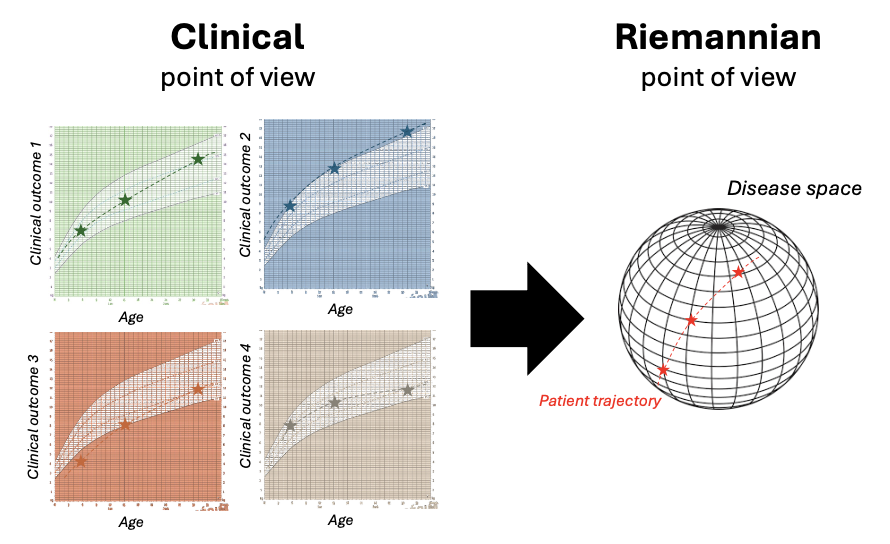
\includegraphics[width=0.96\linewidth]{figures/riemannian_pov.png}
    \end{column}
    \begin{column}{0.35\textwidth}
      \begin{itemize}
        \item \textbf{Clinical view:} one curve per outcome against age.
        \item \textbf{Riemannian view:} their joint evolution is one path $\gamma_i$ in disease space.
        %\item Each normalised outcome follows a bounded logistic trajectory.
      \end{itemize}
    \end{column}
  \end{columns}

  \vspace{0.3em}
  \takeaway{Leaspy represents several clinical scores through bounded logistic trajectories.}
  \slidesource{Figure: \textcite{ortholand2024phd}; disease course mapping: \textcite{schiratti2017bayesian}.}
\end{frame}

\begin{frame}{Nonlinear mixed effects: population and individual}
  \begin{columns}[T,onlytextwidth]
    \begin{column}{0.3\textwidth}
      \softbox{softgrey}{
        \centering\textbf{Fixed effects: shared by the cohort} ($g, v_0, t_0, \sigma_\tau, \sigma_\xi$)
      }
    \end{column}
    \begin{column}{0.66\textwidth}
      \softbox{softred}{
        \centering\textbf{Random effects: one set per patient} ($\tau_i, \xi_i, \mathbf w_i$, $\mathbf \zeta_i$)
      }
    \end{column}
  \end{columns}
  
  \centering
  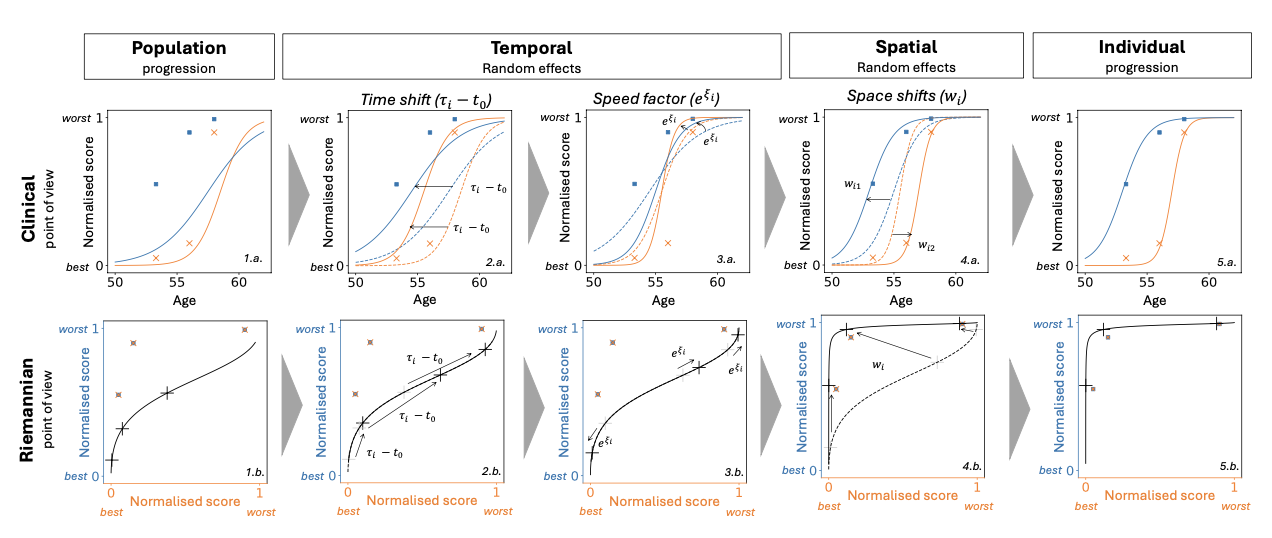
\includegraphics[width=\textwidth]{figures/random_effects.png}

  \slidesource{Figure adapted from \textcite{koval2021ad}.}

\end{frame}

\begin{frame}{Disease age separates disease stage from chronological age}

  \centering
  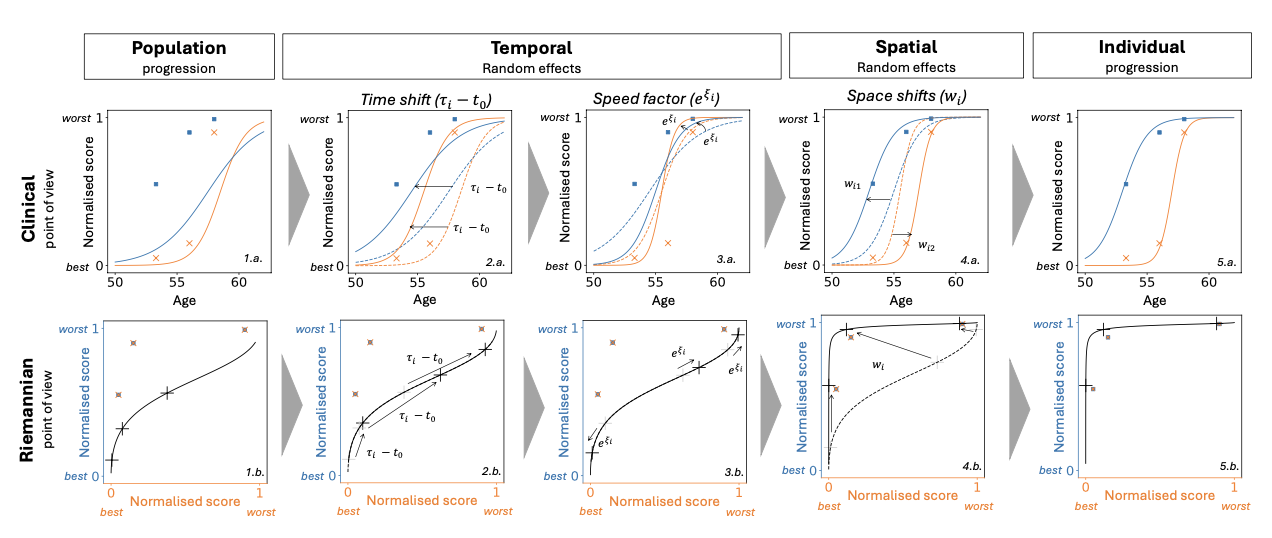
\includegraphics[width=\textwidth]{figures/random_effects.png}
  \vspace*{-1em}
  {\LARGE
    \[
      \boxed{\psi_i(t)=e^{\xi_i}(t-\tau_i)+t_0}
    \]
  }

  \small $\psi_i(t)$ is the latent disease age of patient $i$ at chronological age $t$;
  $\tau_i$ is the individual reference age and $\xi_i$ the log-acceleration.

  \slidesource{Figure adapted from \textcite{koval2021ad}.}
\end{frame}

\begin{frame}{How random effects personalise the trajectory}
  \centering
  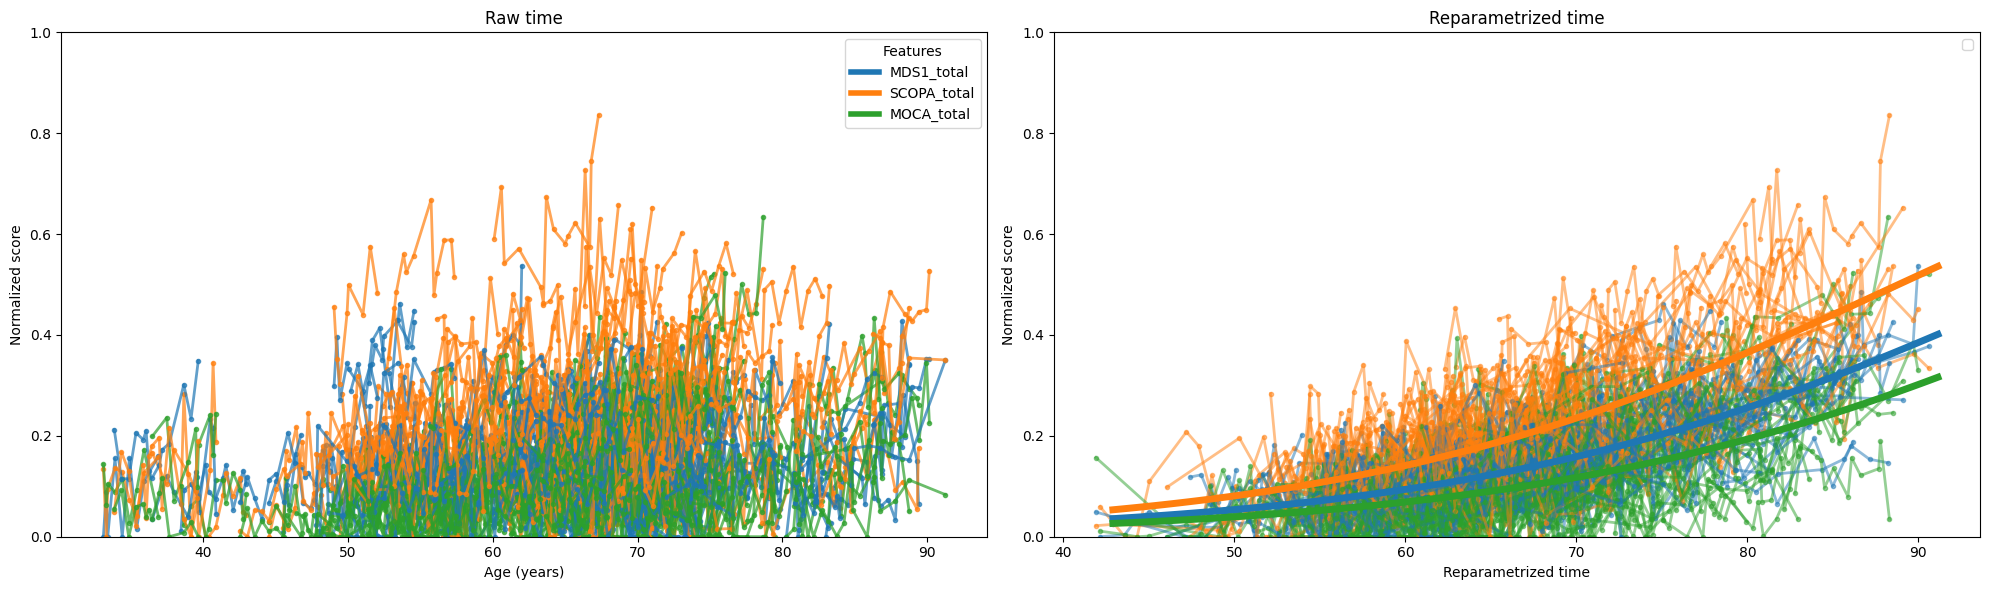
\includegraphics[width=\textwidth]{figures/reparam_time.png}
  \begin{columns}[T,onlytextwidth]
    \begin{column}{0.31\textwidth}
      \softbox{softgrey}{
        \centering
        $\tau_i$\\[0.25em] 
        \small individual reference age; shifts the trajectory earlier or later
      }
    \end{column}
    \begin{column}{0.31\textwidth}
      \softbox{softred}{
        \centering
        $e^{\xi_i}$\\[0.25em]
        \small accelerates or slows disease progression
      }
    \end{column}
    \begin{column}{0.31\textwidth}
      \softbox{softgreen}{
        \centering
        $t_0$\\[0.25em]
        \small anchors the population disease timeline
      }
    \end{column}
  \end{columns}

  \vspace{0.2em}
  \takeaway{Time shift, acceleration, and space shifts transform one population curve into an individual course.}
  \slidesource{Individual disease-course transformations: \textcite{koval2021ad}.}
\end{frame}

\begin{frame}{The joint model: one disease age, two processes}
  \centering
  \resizebox{0.96\linewidth}{!}{%
  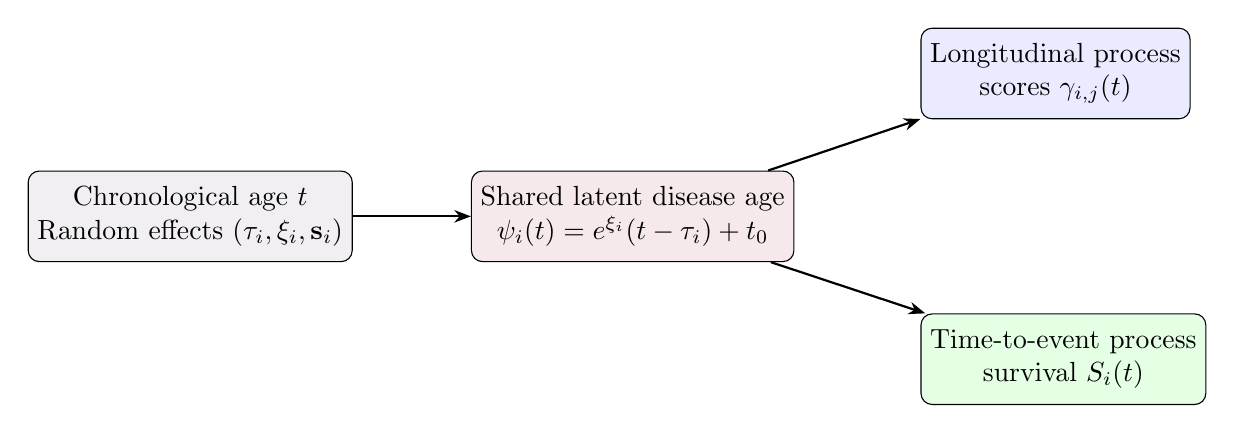
\begin{tikzpicture}[
      node distance=1.15cm and 1.5cm,
      box/.style={draw,rounded corners=4pt,minimum width=3.4cm,minimum height=1.15cm,align=center},
      arr/.style={-{Stealth[length=6pt]},thick}
    ]
    \node[box,fill=CSgrey!12] (patient) {Chronological age $t$\\Random effects $(\tau_i,\xi_i,\mathbf s_i)$};
    \node[box,fill=CSred!10,right=of patient] (psi) {Shared latent disease age\\$\psi_i(t)=e^{\xi_i}(t-\tau_i)+t_0$};
    \node[box,fill=blue!8,above right=0.65cm and 1.6cm of psi] (long) {Longitudinal process\\scores $\gamma_{i,j}(t)$};
    \node[box,fill=green!10,below right=0.65cm and 1.6cm of psi] (surv) {Time-to-event process\\survival $S_i(t)$};
    \draw[arr] (patient) -- (psi);
    \draw[arr] (psi) -- (long);
    \draw[arr] (psi) -- (surv);
  \end{tikzpicture}}

  \vspace{0.7em}
  \begin{itemize}
    \item \textbf{Competing events:} several mutually exclusive outcomes can end follow-up;
      observing one prevents the others from being observed for that patient.
    \item \textbf{Informative dropout:} follow-up ends for a reason related to the patient's
      unobserved health state, so the missing data are not independent of disease progression.
  \end{itemize}
  \slidesource{Joint latent-disease-age models: \textcite{ortholand2025multijoint,ortholand2026joint}.}
\end{frame}

% ============================================================================
\section{How the cohorts are simulated with the joint model}

\begin{frame}[plain,noframenumbering]
  \sectiondividercontent{3}{How the cohorts are simulated with the joint model}
\end{frame}

\begin{frame}{Two input layers must remain distinct}
  \begin{columns}[T,onlytextwidth]
    \begin{column}{0.48\textwidth}
      \softbox{fitinput}{
        \centering\textbf{Learned by \texttt{fit}}
      }
      \begin{itemize}
        \item longitudinal shape: $\fitparam{t_0,\mathbf g,\mathbf v_0}$
        \item heterogeneity: $\fitparam{\sigma_\tau,\sigma_\xi}$
        \item observation noise
        \item survival: $\fitparam{\boldsymbol\nu,\boldsymbol\rho}$
        \item source mixing: $\fitparam{\mathbf A,\boldsymbol\zeta}$
      \end{itemize}
    \end{column}
    \begin{column}{0.48\textwidth}
      \softbox{designinput}{
        \centering\textbf{Specified by the user}
      }
      \begin{itemize}
        \item cohort size $\designparam{N}$
        \item first-visit offset: $\designparam{\bar\delta_f,\sigma_{\delta_f}}$
        \item follow-up: $\designparam{\overline T_f,\sigma_{T_f}}$
        \item inter-visit gap: $\designparam{\bar\delta_v,\sigma_{\delta_v}}$
        \item minimum visit spacing
        \item or an explicit DataFrame visit schedule
      \end{itemize}
    \end{column}
  \end{columns}

  \vfill
  \takeaway{The model determines what disease progression looks like; the user determines what the study looks like.}
\end{frame}

\begin{frame}{Simulation algorithm (1/2): create each follow-up}
  \centering
  \normalsize\textbf{For each patient }$i=1,\ldots,\designparam{N}$\textbf{:}

  \vspace{0.25em} 
  \begin{columns}[T,onlytextwidth]
    \begin{column}{0.31\textwidth}  
      \softbox{softgrey}{
        \small\centering\textbf{1. Random effects}\\[0.25em]
        {\scriptsize draw patient-specific effects}\\[0.1em]
        $\xi_i\sim\mathcal N(0,\fitparam{\sigma_\xi^2})$\\
        $\tau_i\sim\mathcal N(\fitparam{t_0},\fitparam{\sigma_\tau^2})$\\[0.15em]
        {\scriptsize plus latent sources, when present} 
      }
    \end{column}
    \begin{column}{0.31\textwidth}
      \softbox{softred}{
        \small\centering\textbf{2. First visit}\\[0.25em]
        {\scriptsize draw the first-visit time}\\[0.1em]
        $t_{i,0}=\tau_i+\designparam{\delta_{f_i}}$\\
        $\delta_{f_i}\sim\mathcal N(\designparam{\bar\delta_f},\designparam{\sigma_{\delta_f}^2})$
      }
    \end{column}
    \begin{column}{0.31\textwidth}
      \softbox{softgreen}{
        \small\centering\textbf{3. Visit schedule}\\[0.25em]
        {\scriptsize draw inter-visit gaps}\\[-0.05em]
        $\delta_{v_{i,r}}\sim\mathcal N(\designparam{\bar\delta_v},\designparam{\sigma_{\delta_v}^2})$\\[0.1em]
        {\scriptsize until the follow-up duration}\\[-0.05em]
        $T_{f_i}\sim\mathcal N(\designparam{\overline T_f},\designparam{\sigma_{T_f}^2})$
      }
    \end{column}
  \end{columns}

  \vspace{0.35em}
  \centering
  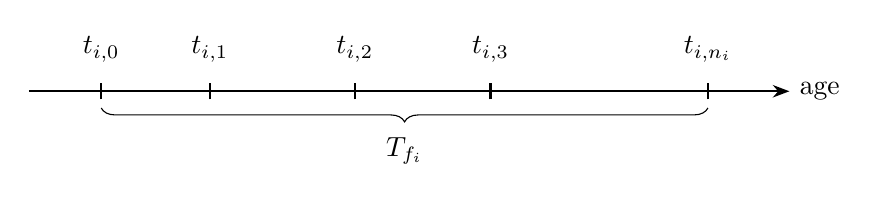
\begin{tikzpicture}[x=1.15cm,y=0.85cm]
    \draw[-{Stealth[length=6pt]},thick] (0,0)--(8.4,0) node[right]{age};
    \foreach \x/\lab in {0.8/$t_{i,0}$,2.0/$t_{i,1}$,3.6/$t_{i,2}$,5.1/$t_{i,3}$,7.5/$t_{i,n_i}$}{
      \draw[thick] (\x,-0.12)--(\x,0.12) node[above=4pt]{\lab}; 
    }
    \draw[decorate,decoration={brace,mirror,amplitude=5pt}] (0.8,-0.25)--(7.5,-0.25)
      node[midway,below=7pt]{$T_{f_i}$};
  \end{tikzpicture}

  \vspace{0.15em}
  \takeaway{Steps 2--3 are governed by the user-defined study design.}
\end{frame}

\begin{frame}{Simulation algorithm (2/2): outcomes and events}
  \centering
  \normalsize\textbf{For each patient }$i=1,\ldots,\designparam{N}$\textbf{:}

  \vspace{0.25em}
  \begin{columns}[T,onlytextwidth]
    \begin{column}{0.31\textwidth}
      \softbox{softgrey}{
        \small\centering\textbf{4. Outcomes}\\[0.25em]
        {\scriptsize compute disease age and trajectory}\\[0.1em]
        $\psi_i(t_{i,r}),\ \gamma_i$\\[0.15em]
        {\scriptsize draw bounded observations with Beta noise}
      }
    \end{column}
    \begin{column}{0.31\textwidth}
      \softbox{softred}{
        \small\centering\textbf{5. Event time}\\[0.25em]
        {\scriptsize inverse-transform sampling from survival}\\[0.1em]
        $T_{e_i}\sim e^{-\xi_i}\mathcal W(\fitparam{\nu},\fitparam{\rho})+\tau_i$
      }
    \end{column}
    \begin{column}{0.31\textwidth}
      \softbox{softgreen}{
        \small\centering\textbf{6. Censoring}\\[0.25em]
        {\scriptsize remove visits after $T_{e_i}$}\\[0.15em]
        {\scriptsize right-censor events beyond the final visit}
      }
    \end{column}
  \end{columns}

  \vspace{0.35em}
  \centering
  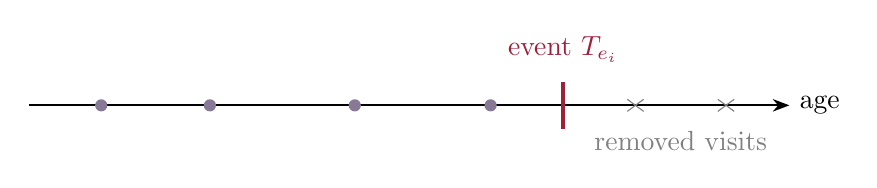
\begin{tikzpicture}[x=1.15cm,y=0.85cm]
    \draw[-{Stealth[length=6pt]},thick] (0,0)--(8.4,0) node[right]{age};
    \foreach \x in {0.8,2.0,3.6,5.1}{\fill[CSgrey] (\x,0) circle (2.2pt);}
    \draw[CSred,very thick] (5.9,-0.35)--(5.9,0.35) node[above=3pt]{event $T_{e_i}$};
    \foreach \x in {6.7,7.7}{
      \draw[gray] (\x-0.09,-0.09)--(\x+0.09,0.09);
      \draw[gray] (\x-0.09,0.09)--(\x+0.09,-0.09);
    }
    \node[gray,below=6pt] at (7.2,0){removed visits};
  \end{tikzpicture}

  \vspace{0.15em}
  \takeaway{Output: longitudinal observations, an event or censoring time, and its indicator.}
\end{frame}

\begin{frame}{Integrating joint simulation inside Leaspy}  
  \centering
  \resizebox{\linewidth}{!}{%
  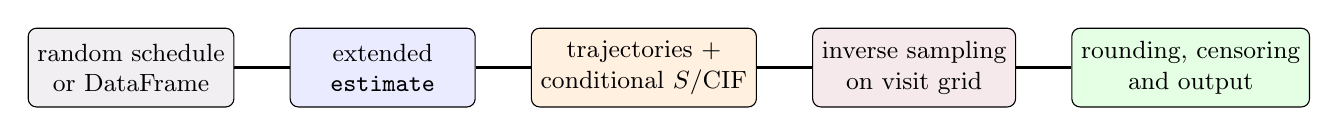
\begin{tikzpicture}[
      node distance=0.7cm,
      box/.style={draw,rounded corners=3pt,minimum width=2.35cm,minimum height=1.0cm,align=center,font=\small},
      link/.style={thick}
    ]
    \node[box,fill=CSgrey!12] (visits) {random schedule\\or DataFrame};
    \node[box,fill=blue!8,right=of visits] (estimate) {extended\\\texttt{estimate}};
    \node[box,fill=orange!12,right=of estimate] (cond) {trajectories +\\conditional $S$/CIF};
    \node[box,fill=CSred!10,right=of cond] (sample) {inverse sampling\\on visit grid};
    \node[box,fill=green!10,right=of sample] (output) {rounding, censoring\\and output};
    \draw[link] (visits)--(estimate);
    \draw[link] (estimate)--(cond);
    \draw[link] (cond)--(sample);
    \draw[link] (sample)--(output);
  \end{tikzpicture}}

  \vspace{0.7em}
  \begin{columns}[T,onlytextwidth]
    \begin{column}{0.48\textwidth}
      \softbox{softgrey}{
        \textbf{1. Standard workflow}\\[0.25em]
        Extend \texttt{estimate} so joint models can use the same
        \texttt{simulate} workflow as other Leaspy models.
      }
    \end{column}
    \begin{column}{0.48\textwidth}
      \softbox{softred}{
        \textbf{2. Competing events}\\[0.25em]
        Generalise event prediction and sampling from one event to several competing event types.
      }
    \end{column}
  \end{columns}

  \vspace{0.5em}
  \centering\scriptsize
  \softbox{softgreen}{The other adaptations are mainly developer/API-oriented considerations and are detailed in the appendix.}
\end{frame}

% ============================================================================
\section{How the self-consistency of the simulation is tested}

\begin{frame}[plain,noframenumbering]
  \sectiondividercontent{4}{How the self-consistency of the simulation is tested}
\end{frame}

\begin{frame}{How simulation quality is assessed}
  \centering
  \validationdiagram{1}
\end{frame}

\begin{frame}{What is simulated exactly?}
  \softbox{softgrey}{
    \centering
    Reference: multivariate joint model fitted on the PRO-ACT ALS dataset\\
    $J=4$ longitudinal features, $K=2$ latent sources, $L=1$ event (death)
  }

  \vspace{0.6em}
  \begin{columns}[T,onlytextwidth]
    \begin{column}{0.48\textwidth}
      \begin{block}{Bulbar function}
        Speech, salivation, and swallowing items.
      \end{block}
      \begin{block}{Fine-motor function}
        Handwriting; cutting food/handling utensils; dressing and hygiene.
      \end{block}
    \end{column}
    \begin{column}{0.48\textwidth}
      \begin{block}{Gross-motor function}
        Turning in bed; walking; climbing stairs.
      \end{block}
      \begin{block}{Total function}
        Overall ALSFRS-R: all items, including the preceding domains and respiratory items.
      \end{block}
    \end{column}
  \end{columns}

  %\vfill
  %\scriptsize Respiratory items: dyspnea, orthopnea, and respiratory insufficiency.
\end{frame}

\begin{frame}{Step 1: simulate from a known reference model}
  \centering
  \validationdiagram{2}
\end{frame}

\begin{frame}{Step 2: fit a fresh model to each synthetic cohort}
  \centering
  \validationdiagram{3}
\end{frame}

\begin{frame}{Experimental setting: deliberately information-rich}
  \begin{columns}[T,onlytextwidth]
    \begin{column}{0.31\textwidth}
      \softbox{softgrey}{
        \centering\textbf{Replications}\\[0.5em]
        $N=1000$ patients\\
        $M=200$ cohorts
      }
    \end{column}
    \begin{column}{0.31\textwidth}
      \softbox{softred}{
        \centering\textbf{Visit process}\\[0.5em]
        first offset $-2\pm1$ y\\
        follow-up $6\pm2$ y\\
        interval $0.083\pm0.042$ y\\
        minimum $0.05$ y
      }
    \end{column}
    \begin{column}{0.31\textwidth}
      \softbox{softgreen}{
        \centering\textbf{Estimation}\\[0.5em]
        MCMC-SAEM\\
        $70\,000$ fit iterations\\
        $5\,000$ personalisation iterations
      }
    \end{column}
  \end{columns}

  \vspace{1.2em}
  \softbox{softred}{
    \centering
    \textbf{Interpretation boundary:} short visit intervals and long follow-up create a favourable dense-observation setting.
  }

  \vfill
  \slidesource{MCMC-SAEM for nonlinear mixed-effects models: \textcite{kuhn2005maximum}.}
\end{frame}

\begin{frame}{Step 3: retain and recover individual effects}
  \centering
  \validationdiagram{4}
\end{frame}

\begin{frame}{Step 4: compare population and individual recovery}
  \centering
  \validationdiagram{5}
\end{frame}

\begin{frame}{Four recovery metrics, two inference levels}
  \begin{columns}[T,onlytextwidth]
    \begin{column}{0.49\textwidth}
      \softbox{softgrey}{
        \centering\textbf{Fixed effects / population parameters}
      }
      \vspace{0.4em}
      \footnotesize
      Define the relative error in repetition $m$ as
      \[
        e_m=\frac{\hat\theta^{(m)}-\theta^*}{|\theta^*|}\times100.
      \]
      \[
        \mathrm{RB}=\frac{1}{M}\sum_{m=1}^{M}e_m
      \]
      signed systematic error; best value: $0\%$.

      \[
        \mathrm{RRMSE}=\sqrt{\frac{1}{M}\sum_{m=1}^{M}e_m^2}
      \]
      total error from bias and dispersion; best value: $0\%$.
    \end{column}
    \begin{column}{0.47\textwidth}
      \softbox{softred}{
        \centering\textbf{Individual random effects}
      }
      \vspace{0.7em}
      \begin{block}{ICC(3,1)}
        Consistency between true and personalised values while accounting for disagreement beyond rank ordering.
      \end{block}
      \begin{block}{Pearson's $r$}
        Strength of linear association; invariant to location and scale changes.
      \end{block}
      \centering
      Best value for both: $1$.
    \end{column}
  \end{columns}
\end{frame}

\begin{frame}{The complete self-consistency experiment}
  \centering
  \validationdiagram{5}

  \vspace{0.5em}
  \takeaway{Self-consistency asks whether the model can recover what it generated.}
\end{frame}

\section{Results of the experiments}

\begin{frame}[plain,noframenumbering]
  \sectiondividercontent{5}{Results of the experiments}
\end{frame}

\begin{frame}{Fixed effects / population parameters: recovery}
  \centering
  \small
  \setlength{\tabcolsep}{4.5pt}
  \renewcommand{\arraystretch}{1.28}
  \resizebox{\linewidth}{!}{%
  \begin{tabular}{lclcc}
    \toprule
    Component & Parameters & Interpretation & RB (\%) & RRMSE (\%)\\
    \midrule
    Temporal & $t_0,\sigma_\tau,\sigma_\xi$ & reference and variability
      & $0.03$ to $0.44$ & $0.83$ to $2.32$\\
    Survival & $\rho,\nu$ & Weibull shape and scale
      & $0.10$ to $2.33$ & $5.01$ to $5.43$\\
    Noise & $\sigma^{(0:3)}$ & observation noise
      & $-4.60$ to $-1.26$ & $1.47$ to $4.73$\\
    Position & $g^{(0:3)}$ & logistic position
      & $-8.80$ to $-5.92$ & $8.09$ to $12.61$\\
    Velocity & $v_0^{(0:3)}$ & logistic velocity
      & $1.12$ to $6.46$ & $4.52$ to $10.53$\\
    \bottomrule
  \end{tabular}}

  \vspace{0.9em}
  \begin{columns}[T,onlytextwidth]
    \begin{column}{0.48\textwidth}
      \softbox{softgreen}{
        \textbf{Best recovered:} temporal population parameters, supported by many repeated observations per patient.
      }
    \end{column}
    \begin{column}{0.48\textwidth}
      \softbox{softred}{
        \textbf{Hardest:} trajectory positions $g$ and bulbar velocity $v_0^{(0)}$, which can compensate for each other.
      }
    \end{column}
  \end{columns}
\end{frame}

\begin{frame}{Individual random effects: recovery (1/2)}
  \begin{columns}[T,onlytextwidth]
    \begin{column}{0.59\textwidth}
      \centering
      \small
      \renewcommand{\arraystretch}{1.23}
      \begin{tabular}{lcc}
        \toprule
        Effect & ICC(3,1) & Pearson's $r$\\
        \midrule
        $\xi_i$ & $0.988\pm0.004$ & $0.989\pm0.004$\\
        $\tau_i$ & $0.995\pm0.002$ & $0.995\pm0.002$\\
        $w_{i,0}$ & $0.987\pm0.006$ & $0.992\pm0.003$\\
        $w_{i,1}$ & $0.989\pm0.003$ & $0.990\pm0.003$\\
        $w_{i,2}$ & $0.990\pm0.003$ & $0.991\pm0.003$\\
        $w_{i,3}$ & $0.987\pm0.003$ & $0.988\pm0.003$\\
        $(\boldsymbol\zeta^\top\mathbf s_i)_0$
          & $0.965\pm0.027$ & $0.978\pm0.013$\\
        \bottomrule
      \end{tabular}

      \vspace{0.3em}
      \scriptsize Mean $\pm$ standard deviation across repetitions.
    \end{column}
    \begin{column}{0.38\textwidth}
      \softbox{softgreen}{
        \textbf{Strong agreement} for every evaluated individual effect: all ICCs exceed $0.96$.
      }

      \vspace{0.7em}
      \softbox{softred}{  
        The \textbf{survival shift} is least precise: it is informed by at most one possibly censored event per patient.
      }

      \vspace{0.7em}
      \scriptsize Source coordinates $\mathbf s_i$ are rotation-dependent, so invariant feature shifts
      $\mathbf w_i=\mathbf A\mathbf s_i$ and survival shifts are compared instead.
    \end{column}
  \end{columns}
\end{frame}

\begin{frame}{Individual random effects: recovery (2/2)}
  \centering
  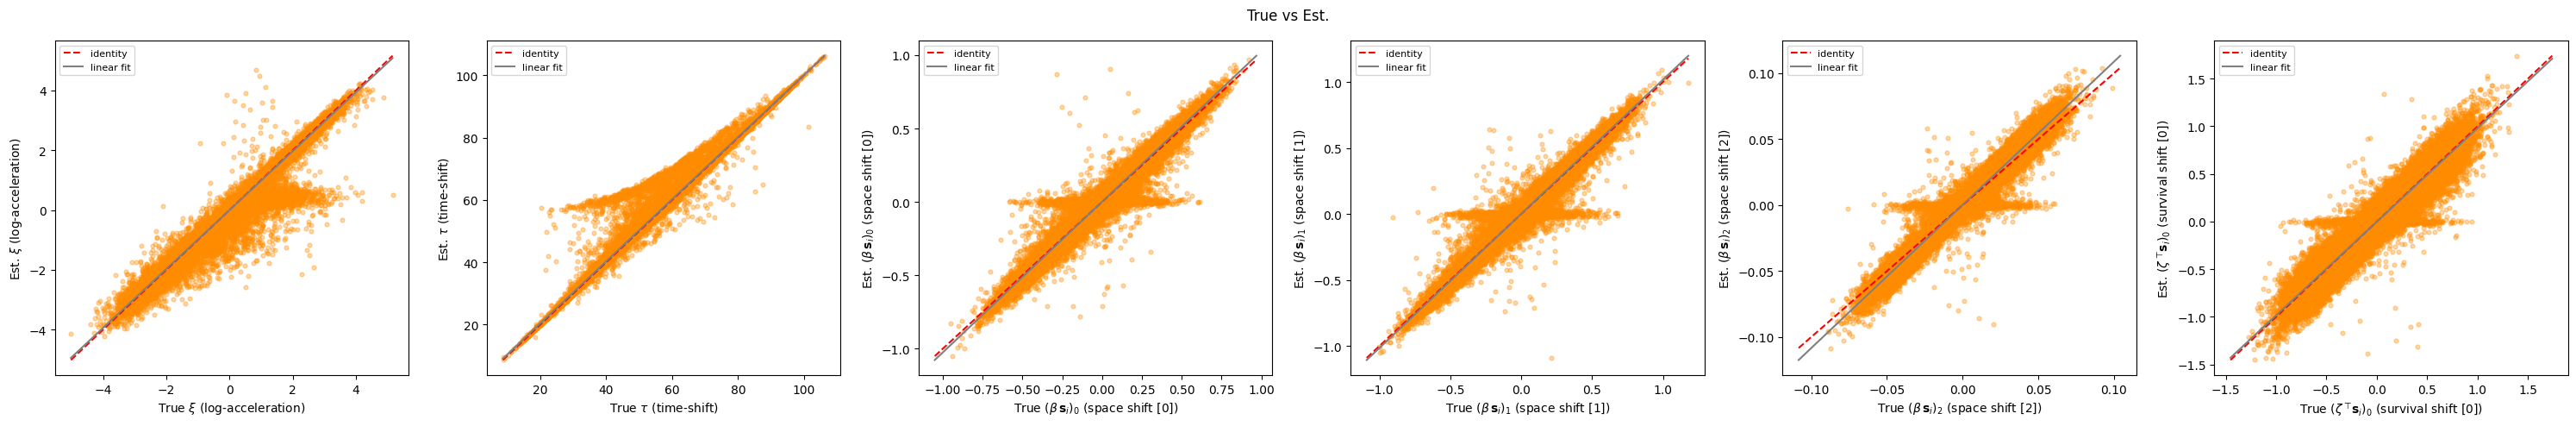
\includegraphics[width=0.86\textwidth,height=0.56\textheight,keepaspectratio]{figures/Indiv_multivariate.png}

  \softbox{softred}{
    \centering\small Aggregate ICC is high, but some low-information patients are pulled toward the population mean.
  }

  \scriptsize True sampled values (x-axis) vs personalised estimates (y-axis). Dashed red: identity;
  grey: linear fit. Points are pooled over patients and repetitions.
\end{frame}

% ============================================================================
\section{Conclusions}

\begin{frame}[plain,noframenumbering]
  \sectiondividercontent{6}{Conclusions}
\end{frame}

\begin{frame}{Take-home messages}
  \softbox{softgrey}{
    \centering
    \textbf{Goal:} integrate joint simulation in Leaspy, then test the complete
    simulate--fit--personalise loop.
  }

  \vspace{0.6em}
  \small
  \begin{enumerate}
    \item \textbf{Integration achieved:} joint simulation now uses the standard Leaspy API,
      including survival, censoring, and competing events.
    \item \textbf{Validation achieved:} the complete loop is self-consistent in the favourable
      dense setting studied.
    \item \textbf{Main result:} temporal and individual effects are recovered very well;
      trajectory positions and survival-related quantities are less precisely identified.
    \item \textbf{Scope:} recovery under sparse visits, heavier censoring, or model
      misspecification remains to be evaluated.
  \end{enumerate}

\end{frame}

\begin{frame}{Ethical and sustainability considerations \hfill \CSonly}
  \begin{columns}[T,onlytextwidth]
    \begin{column}{0.31\textwidth}
      \softbox{softgrey}{
        \centering\textbf{Patient privacy}\\[0.45em]
        \small Synthetic cohorts do not correspond to real patients and can facilitate sharing.\\[0.45em]
        They still require clear labelling, provenance, governance, and disclosure-risk assessment.
      }
    \end{column}
    \begin{column}{0.31\textwidth}
      \softbox{softred}{
        \centering\textbf{Computational cost}\\[0.45em]
        \small $200$ fits $\times$ $70\,000$ iterations plus personalisation is not negligible.\\[0.45em]
        Small preliminary runs and saved intermediates avoid unnecessary recomputation.
      }
    \end{column}
    \begin{column}{0.31\textwidth}
      \softbox{softgreen}{
        \centering\textbf{Software responsibility}\\[0.45em]
        \small Errors can propagate into scientific conclusions.\\[0.45em]
        Unit tests, functional tests, documentation, and peer review are part of methodological rigour.
      }
    \end{column}
  \end{columns}

  \vfill
  \takeaway{Synthetic does not mean risk-free, and reproducible does not mean cost-free.}
\end{frame}

\begin{frame}[allowframebreaks]{References}
  \printbibliography[heading=none]
\end{frame}

% ============================================================================
\appendix
\section{Supplementary material}

\begin{frame}{Appendix: notation and normalised disease space}
  \small
  \begin{columns}[T,onlytextwidth]
    \begin{column}{0.47\textwidth}
      \begin{tabular}{>{$}l<{$} @{\hspace{0.8em}} l}
        i=1,\ldots,N & patient\\[0.35em]
        r=1,\ldots,n_i & visit\\[0.35em]
        j=1,\ldots,J & longitudinal feature\\[0.35em]
        k=1,\ldots,K & latent source\\[0.35em]
        l=1,\ldots,L & event type
      \end{tabular}
    \end{column}
    \begin{column}{0.49\textwidth}
      \begin{itemize}
        \item $t_{i,r,j}$: chronological age
        \item $y_{i,r,j}$: observed score
        \item $\gamma_{i,j}$: latent individual trajectory
        \item $\epsilon_{i,r,j}$: observation noise
      \end{itemize}
    \end{column}
  \end{columns}

  \vspace{0.9em}
  \softbox{softgrey}{
    With $J$ normalised clinical scores, the disease space is $(0,1)^J$.
    The chosen metric produces bounded logistic trajectories in this space.
  }

  \vspace{0.6em}
  \centering
  $y_{i,r,j}=\gamma_{i,j}(t_{i,r,j})+\epsilon_{i,r,j}$
\end{frame}

\begin{frame}{Appendix: why the metric produces a logistic trajectory}
  \scriptsize
  \setlength{\abovedisplayskip}{0.35em}
  \setlength{\belowdisplayskip}{0.35em}
  \begin{columns}[T,onlytextwidth]
    \begin{column}{0.48\textwidth}
      \softbox{softgrey}{
        \textbf{1. Flatten the Riemannian geometry}\par
        For one score, let $M=(0,1)$ with
        \[
          \mathrm ds^2=G(p)\,\mathrm dp^2,
          \qquad G(p)=\frac{1}{p^2(1-p)^2}.
        \]
        Define the logit coordinate
        \[
          \phi(p)=\log\!\frac{p}{1-p},
          \qquad \phi'(p)=\frac{1}{p(1-p)}.
        \]
        Since $\phi'(p)^2=G(p)$, we obtain
        $\mathrm ds^2=\mathrm d\phi^2$: the geometry is Euclidean
        in the $\phi$ coordinate.
      }

      \vspace{0.55em}
      \textbf{2. Geodesics become straight lines}\par
      Therefore a geodesic $\gamma$ satisfies
      \[
        \phi(\gamma(t))=\phi(p_0)+c(t-t_0).
      \]
    \end{column}

    \begin{column}{0.48\textwidth}
      \textbf{3. Map back to $(0,1)$}\par
      Applying the inverse logit gives
      \[
        \gamma(t)=
        \left[1+\frac{1-p_0}{p_0}
        e^{-c(t-t_0)}\right]^{-1},
      \]
      which is a bounded logistic trajectory.

      \vspace{0.55em}
      \softbox{softgrey}{
        \textbf{4. Recover Leaspy's parametrisation}\par
        Set $p_0=1/(1+g)$ and require
        $\dot\gamma(t_0)=v_0$. Because
        $\dot\gamma=c\gamma(1-\gamma)$,
        \[
          c=\frac{v_0}{p_0(1-p_0)}
           =\frac{(1+g)^2}{g}v_0.
        \]
      }
    \end{column}
  \end{columns}

  \vspace{0.35em}
  \[
    \boxed{\gamma(t)=\left[1+g\exp\!\left(
      -\frac{(1+g)^2}{g}v_0(t-t_0)\right)\right]^{-1}}
  \]
  \vspace{-0.2em}
  \takeaway{A straight geodesic in logit coordinates becomes a logistic curve in score space.}
\end{frame}

\begin{frame}{Appendix: full longitudinal model}
  \footnotesize
  \[
  \left\{
  \begin{aligned}
    \psi_i(t) &= e^{\xi_i}(t-\tau_i)+t_0,\\
    \mathbf w_i &= \mathbf A\mathbf s_i,\\
    \gamma_{i,j}(t)
      &=\left[1+g_j\exp\!\left(-\frac{(1+g_j)^2}{g_j}
        \left(v_{0,j}(\psi_i(t)-t_0)+w_{i,j}\right)\right)\right]^{-1},\\
    y_{i,r,j} &= \gamma_{i,j}(t_{i,r,j})+\epsilon_{i,r,j},
      \qquad \epsilon_{i,r,j}\sim\mathcal N(0,\sigma_j^2).
  \end{aligned}
  \right.
  \]

  \vspace{0.8em}
  \begin{itemize}
    \item $p_j=1/(1+g_j)$ is the population trajectory value at $t_0$.
    \item $v_{0,j}$ controls the velocity at the reference time.
    \item $w_{i,j}$ changes the relative ordering of feature trajectories.
  \end{itemize}
\end{frame}

\begin{frame}{Appendix: survival and latent-source coupling}
  \footnotesize
  \begin{block}{Single-event survival on disease age}
    \[
      S_i(t)=\mathbf 1_{\psi_i(t)>t_0}
      \exp\!\left[-\left(\frac{\psi_i(t)-t_0}{\nu}\right)^\rho\right]
      +\mathbf 1_{\psi_i(t)\le t_0}.
    \]
  \end{block}

  \begin{block}{Event-specific scale with sources}
    For event $l$,
    \[
      \nu_{i,l}=\nu_l\exp\!\left[-\xi_i-
      \frac{1}{\rho_l}(\boldsymbol\zeta^\top\mathbf s_i)_l\right].
    \]
  \end{block}

  \begin{itemize}
    \item Each competing event has its own Weibull pair $(\nu_l,\rho_l)$.
    \item $\mathrm{CIF}_{i,l}(t)$ gives the probability that cause $l$ has occurred by $t$ in the presence of competing causes.
  \end{itemize}
\end{frame}

\begin{frame}{Appendix: discrete event sampling in Leaspy}
  \small
  \[
  F_i^{\mathrm{cond}}(t_{i,r})=
  \begin{cases}
    1-S_i(t_{i,r})/S_i(t_{i,0}), & \text{single event},\\[0.5em]
    \displaystyle\sum_{l=1}^{L}\mathrm{CIF}_{i,l}(t_{i,r})/S_i(t_{i,0}),
      & \text{competing events}.
  \end{cases}
  \]

  \begin{enumerate}
    \item Draw $U\sim\mathcal U[0,1]$.
    \item Select the first planned visit where $F_i^{\mathrm{cond}}(t_{i,r})\ge U$.
    \item If no visit crosses $U$, right-censor at the last visit.
    \item For competing risks, sample the cause from incremental cause-specific CIFs.
  \end{enumerate}

  \takeaway{This ensures internal API reuse, but discretises event times onto the visit grid.}
\end{frame}

\begin{frame}{Appendix: additional Leaspy adaptations}
  \begin{block}{Visit schedules and study parameters}
    The simulator accepts either a random visit process or a user-provided schedule.
    Missing random-mode study parameters can be estimated from an input dataset.
  \end{block}

  \begin{block}{Bounded observation noise}
    Longitudinal observations use Beta noise. Near score boundaries, an infeasible variance
    is clamped to $0.99\,\mu(1-\mu)$ and a warning identifies the affected observation.
  \end{block}

  \begin{block}{Competing causes and rounding}
    Event types are sampled from incremental cause-specific cumulative incidences.
    After visit-time rounding, a final censoring pass removes any visit moved beyond the event time.
  \end{block}
\end{frame}

\begin{frame}{Appendix: detailed population recovery (1/2)}
  \centering
  \scriptsize
  \renewcommand{\arraystretch}{1.18}
  \resizebox{\linewidth}{!}{%
  \begin{tabular}{lrrrrr}
    \toprule
    Parameter & $\theta^*$ & $\bar{\hat\theta}$ & RB (\%) [95\% CI] & RRMSE (\%) [95\% CI] & RSE [95\% CI]\\
    \midrule
    $g^{(0)}$    & $10.461$ & $9.595$ & $-8.27\ [-9.41,-7.23]$ & $11.41\ [10.60,12.28]$ & $0.086\ [0.076,0.095]$\\
    $g^{(1)}$    & $2.326$  & $2.122$ & $-8.80\ [-10.03,-7.52]$ & $12.61\ [11.55,13.66]$ & $0.099\ [0.087,0.111]$\\
    $g^{(2)}$    & $1.951$  & $1.803$ & $-7.60\ [-8.71,-6.52]$ & $11.16\ [10.26,12.06]$ & $0.089\ [0.079,0.098]$\\
    $g^{(3)}$    & $3.415$  & $3.213$ & $-5.92\ [-6.68,-5.17]$ & $8.09\ [7.46,8.76]$ & $0.059\ [0.052,0.066]$\\
    $v_0^{(0)}$ & $0.078$  & $0.083$ & $6.46\ [5.32,7.65]$ & $10.53\ [9.56,11.53]$ & $0.078\ [0.070,0.086]$\\
    $v_0^{(1)}$ & $0.257$  & $0.263$ & $2.23\ [1.54,2.93]$ & $5.57\ [5.05,6.12]$ & $0.050\ [0.045,0.054]$\\
    $v_0^{(2)}$ & $0.238$  & $0.241$ & $1.12\ [0.52,1.74]$ & $4.52\ [4.12,4.92]$ & $0.043\ [0.039,0.047]$\\
    $v_0^{(3)}$ & $0.133$  & $0.135$ & $2.05\ [1.37,2.73]$ & $5.25\ [4.75,5.78]$ & $0.048\ [0.043,0.052]$\\
    \bottomrule
  \end{tabular}}

  \vspace{0.8em}
  \softbox{softgrey}{
    \footnotesize Intervals are 95\% percentile bootstrap confidence intervals from 2,000 resamples of the $M=200$ cohort-level estimates.
  }
\end{frame}

\begin{frame}{Appendix: detailed population recovery (2/2)}
  \centering
  \scriptsize
  \renewcommand{\arraystretch}{1.15}
  \resizebox{\linewidth}{!}{%
  \begin{tabular}{lrrrrr}
    \toprule
    Parameter & $\theta^*$ & $\bar{\hat\theta}$ & RB (\%) [95\% CI] & RRMSE (\%) [95\% CI] & RSE [95\% CI]\\
    \midrule
    $\rho$         & $1.849$  & $1.851$  & $0.10\ [-0.61,0.81]$ & $5.01\ [4.50,5.51]$ & $0.050\ [0.045,0.055]$\\
    $\nu$          & $4.047$  & $4.142$  & $2.33\ [1.64,3.00]$ & $5.43\ [4.97,5.91]$ & $0.048\ [0.043,0.053]$\\
    $\sigma^{(0)}$ & $0.069$  & $0.065$  & $-4.60\ [-4.76,-4.45]$ & $4.73\ [4.58,4.89]$ & $0.012\ [0.011,0.013]$\\
    $\sigma^{(1)}$ & $0.079$  & $0.075$  & $-4.16\ [-4.28,-4.04]$ & $4.25\ [4.14,4.38]$ & $0.009\ [0.009,0.010]$\\
    $\sigma^{(2)}$ & $0.074$  & $0.072$  & $-3.08\ [-3.17,-2.97]$ & $3.17\ [3.07,3.27]$ & $0.008\ [0.007,0.009]$\\
    $\sigma^{(3)}$ & $0.045$  & $0.044$  & $-1.26\ [-1.37,-1.15]$ & $1.47\ [1.37,1.56]$ & $0.008\ [0.007,0.009]$\\
    $t_0$          & $56.699$ & $56.948$ & $0.44\ [0.35,0.53]$ & $0.83\ [0.76,0.90]$ & $0.007\ [0.006,0.008]$\\
    $\sigma_\tau$ & $11.630$ & $11.639$ & $0.08\ [-0.24,0.38]$ & $2.32\ [2.10,2.54]$ & $0.023\ [0.021,0.025]$\\
    $\sigma_\xi$  & $1.078$  & $1.079$  & $0.03\ [-0.27,0.37]$ & $2.32\ [2.11,2.56]$ & $0.023\ [0.021,0.026]$\\
    \bottomrule
  \end{tabular}}

  \vspace{0.7em}
  \softbox{softgrey}{
    \footnotesize $\theta^*$ is the generating value; $\bar{\hat\theta}$ is the mean estimate across the 200 independently fitted cohorts.
  }
\end{frame}

\begin{frame}{Appendix: population relative-error distributions}
  \centering
  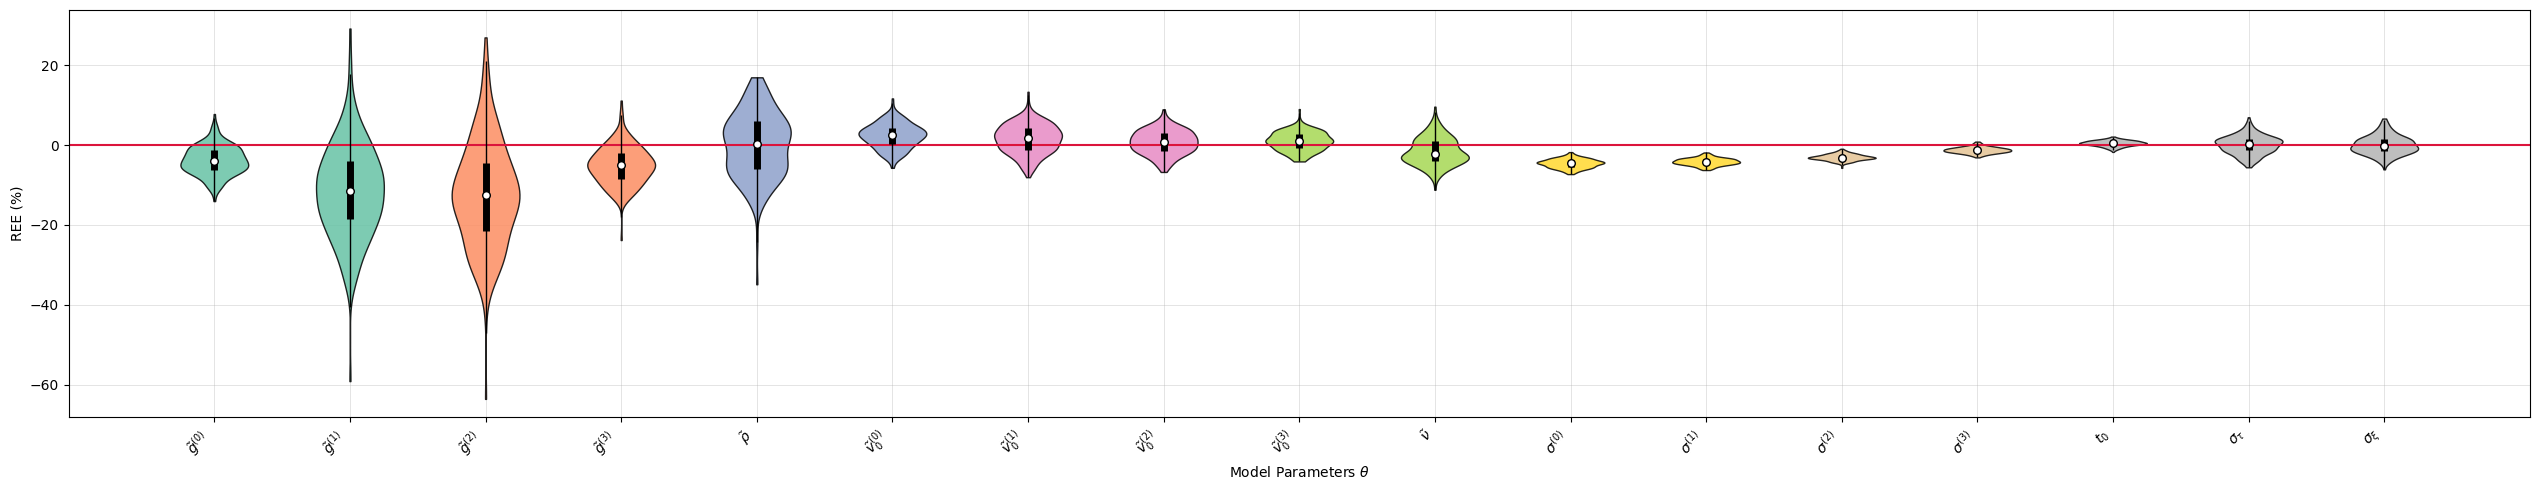
\includegraphics[width=0.96\textwidth,height=0.72\textheight,keepaspectratio]{figures/REE_multivariate.png}

  \scriptsize Red: zero relative error. Temporal parameters concentrate closest to zero;
  trajectory positions $g^{(j)}$ show the largest systematic underestimation.
\end{frame}

\begin{frame}{Appendix: detailed individual-effect recovery}
  \centering
  \small
  \renewcommand{\arraystretch}{1.2}
  \begin{tabular}{lcc}
    \toprule
    Effect & ICC(3,1) & Pearson's $r$\\
    \midrule
    $\xi_i$ & $0.988\pm0.004$ & $0.989\pm0.004$\\
    $\tau_i$ & $0.995\pm0.002$ & $0.995\pm0.002$\\
    $w_{i,0}$ & $0.987\pm0.006$ & $0.992\pm0.003$\\
    $w_{i,1}$ & $0.989\pm0.003$ & $0.990\pm0.003$\\
    $w_{i,2}$ & $0.990\pm0.003$ & $0.991\pm0.003$\\
    $w_{i,3}$ & $0.987\pm0.003$ & $0.988\pm0.003$\\
    $(\boldsymbol\zeta^\top\mathbf s_i)_0$ & $0.965\pm0.027$ & $0.978\pm0.013$\\
    \bottomrule
  \end{tabular}

  \vspace{0.7em}
  \softbox{softgrey}{
    \footnotesize Values are mean $\pm$ standard deviation across the $M=200$ cohorts, as reported in the report.
  }
\end{frame}

\begin{frame}{Appendix: Bland--Altman diagnostic}
  \centering
  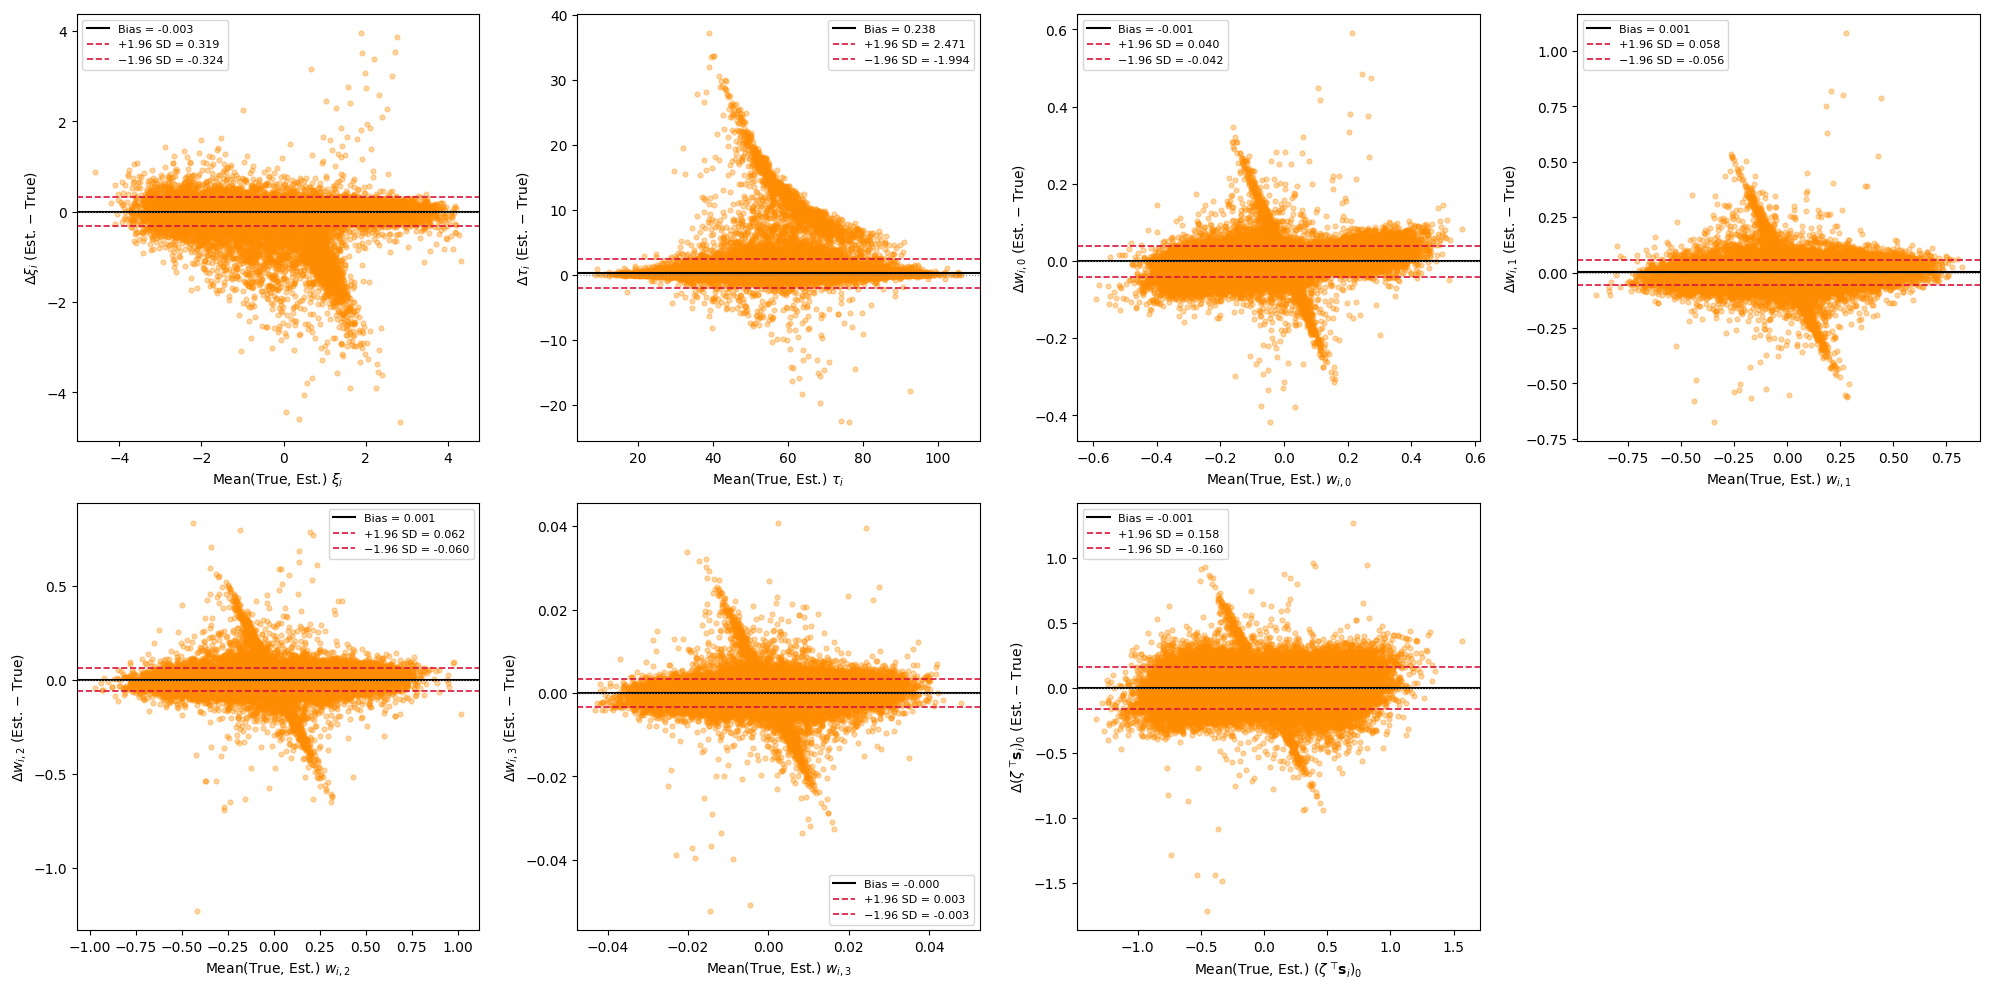
\includegraphics[width=\textwidth]{figures/bland-altman_multivariate.png}

  \scriptsize Black: mean difference; red: limits of agreement. Biases are close to zero for all effects.
\end{frame}

\begin{frame}{Appendix: software-level validation}
  \begin{columns}[T,onlytextwidth]
    \begin{column}{0.48\textwidth}
      \softbox{softgrey}{\centering\textbf{Simulation unit tests}}
      \begin{itemize}
        \item non-empty random-mode output
        \item expected patient count
        \item strictly increasing visit times
        \item DataFrame schedules are respected
        \item all model features are returned
      \end{itemize}
    \end{column}
    \begin{column}{0.48\textwidth}
      \softbox{softred}{\centering\textbf{\texttt{estimate} functional tests}}
      \begin{itemize}
        \item univariate numerical correctness
        \item raw/DataFrame consistency
        \item MultiIndex preservation
        \item multivariate output shape:
          $n_{\mathrm{timepoints}}\times(J+L)$
      \end{itemize}
    \end{column}
  \end{columns}
\end{frame}

\begin{frame}{Appendix: limitations and next experiments}
  \begin{block}{What the reported experiment establishes}
    Self-consistency of the integrated pipeline for $N=1000$ under a favourable, dense visit design.
  \end{block}

  \begin{block}{What it does not establish}
    Universal recovery under sparse visits, heavier censoring, smaller cohorts, or model misspecification.
  \end{block}

  \begin{block}{Perspectives stated in the report}
    Vary sample size, censoring intensity, visit sparsity, and misspecification; explore more flexible visit schedules and noise models; align continuous-time event generation more closely with the grid-based implementation.
  \end{block}
\end{frame}

\begin{frame}{Appendix: results of the original paper's simulation study}
\scriptsize
\centering
\resizebox{\textwidth}{!}{%
\begin{tabular}{lllrr}
\hline
 & Parameters name &  & RB (\%) & RRMSE (\%) \\
\hline
Distribution of random effects
& Estimated reference time (mean) & $t_0$ & 0.10 & 2.23 \\
& Estimated reference time (std) & $\sigma_\tau$ & -1.47 & 4.40 \\
& Individual log-speed factor (std) & $\sigma_\xi$ & 13.21 & 14.85 \\
\hline
Longitudinal fixed effects
& Curve values at $t_0$: $\frac{1}{1+g_k}$ & $g_0$ & -5.35 & 9.28 \\
& & $g_1$ & -8.08 & 11.27 \\
& & $g_2$ & -7.74 & 10.87 \\
& & $g_3$ & -5.93 & 7.71 \\
\cline{2-5}
& Speed of the logistic curves $(v_{0,k})$ & $v_{0,0}$ & -7.04 & 10.87 \\
& & $v_{0,1}$ & -7.43 & 10.64 \\
& & $v_{0,2}$ & -8.89 & 11.27 \\
& & $v_{0,3}$ & -9.34 & 11.21 \\
\cline{2-5}
& Estimated noises $(\sigma_k)$ & $\sigma_0$ & -3.22 & 4.12 \\
& & $\sigma_1$ & -1.08 & 2.44 \\
& & $\sigma_2$ & -0.82 & 2.24 \\
& & $\sigma_3$ & 0.17 & 2.14 \\
\hline
Survival fixed effects
& Weibull scale $(\nu_l)$ & $\nu_0$ & 18.04 & 23.19 \\
& & $\nu_1$ & -0.09 & 9.97 \\
\cline{2-5}
& Weibull shape $(\rho_l)$ & $\rho_0$ & -8.38 & 14.15 \\
& & $\rho_1$ & 10.98 & 19.79 \\
\hline
\end{tabular}%
}
\slidesource{Results are extracted from: \textcite{ortholand2025multijoint}.}
\end{frame}
  

\end{document}
